%%%%%%%%%%%%%%%%%%%%%%%%%%%%%%%%%%%%%%%%%%%%%%%%%%%%%%%%%%%%%%%%%%%%%%%%%%%%%%%%
% coding: utf-8 ;
%
% Slides for a talk given on 2016-10-13 at CrySP at the University of Waterloo
% in Ontario, Canada.
%
% Author: Isis Agora Lovecruft <isis@torproject.org> 0xa3adb67a2cdb8b35
% License: CC-BY-SA
%
% Bio: Isis Agora Lovecruft has been a core developer for The Tor Project since
% 2010, whose current work includes protocols for distributing shared secrets in
% a censorship resistant manner, improvements to Tor's circuit-level
% cryptography, and contributing to the design and implementation of a new
% post-quantum hybrid handshake for Tor.
% 
% Title: Hacks and Improvements for Tor's Circuit-Layer Crypto
% 
% Abstract: Since 2010, various nation state adversaries have been conducting
% active probing and enumeration attacks to attempt to collect all of Tor's
% bridges, the unpublished entrances to the Tor network which are used to
% circumvent online censorship.  Since then, an arms race to distribute the
% bridge addresses to honest clients without these adversaries obtaining them
% has ensued.  The proposed solution uses attribute-based credentials to record
% honest users' good behaviour (i.e. the bridges not being censored/blocked),
% which also serves to effectively lock censoring adversaries out of the
% distribution system.  Even with these measures being implemented, there are
% other schemes for discovering the locations of Tor bridges; these will be
% discussed, as well as a hack that can be done with Tor's circuit-layer
% cryptography to protect against it.  After that, I'll discuss a known tagging
% attack on Tor and a much-needed (and highly custom) authenticating encryption
% cipher to defend against it, as well as the design for a post-quantum hybrid
% Tor handshake I've been working on.
%
%%%%%%%%%%%%%%%%%%%%%%%%%%%%%%%%%%%%%%%%%%%%%%%%%%%%%%%%%%%%%%%%%%%%%%%%%%%%%%%%

\documentclass[9pt,a4paper]{beamer}
%\usetheme[background=dark]{metropolis}
\usetheme{metropolis}

\usepackage[utf8x]{inputenc}
\usepackage[T1]{fontenc}
\usepackage{amsmath}
\usepackage{tikz}
\usetikzlibrary{decorations.pathreplacing}
\usetikzlibrary{shapes,patterns,trees,shadows}
\usetikzlibrary{calc, backgrounds}


\newcommand{\bl}{\color{beamer@asblue}}
\newcommand{\bk}{\color{black}}
\newcommand{\rd}{\color{red}}
\newcommand{\gr}{\color{green}}


\title{Tor's Circuit-Layer Cryptography}
\subtitle{Attacks, Hacks, and Improvements}
\author{Isis Agora Lovecruft \\
  Core Developer, The Tor Project
}
\date{\vspace{3mm} October 13th, 2016}
\institute{University of Waterloo}

\begin{document}
\maketitle


\begin{frame}
  \frametitle{Why should you care about privacy?}
  \begin{quotation}
    ``There is an entire genre of YouTube videos devoted to an experience which
    I'm certain that everyone in this room has had. It entails an individual,
    who, thinking they're alone, engages in some expressive behaviour -- wild
    singing, girating dancing, some mild sexual activity -- only to discover
    that, in fact, they are not alone, that there's a person watching and
    lurking, the discovery of which causes them to immediately cease what
    they're doing in horror. The sense of shame and humiliation in their face is
    palpable: it's the sense of `this is something I'm willing to do only if no
    one else is watching.'  This is the crux of the work on which I have been
    singularly focused for the sixteen months: the question of why privacy matters.'' \\
    \hfill{\raggedright---Glenn Greenwald,
      \href{https://www.youtube.com/watch?v=pcSlowAhvUk}{TED Talk}, October 2014}
  \end{quotation}
\end{frame}


\section{Introduction to Tor}

\begin{frame}{Background: Anonymising proxies}
  \begin{itemize}
    \item Typically application-specific proxies, e.g. HTTP proxies, or
      generic request-based proxies, e.g. SOCKS proxies
    \item Requests to online services come from the proxy 
    \item Users behind the proxy should be indistinguishable
    \item Proxies can be chained together
    \item Various problems:
      \begin{enumerate}
        \item Single point-of-failure
        \item<2-> Relatively trivial to correlate ingoing/outgoing traffic
        \item<3-> (Usually) no crypto protecting the connection between the user and the proxy
      \end{enumerate}
    \item<4-> Can add cryptographic or obfuscational features to the proxy, e.g. The
      Tor Project's ``Pluggable Transports'' \dots
    \item<5-> \dots this (usually) still does not solve problems 1 and 2
  \end{itemize}

  \uncover<6->{
    Designs like anonymising proxies which place ultimate trust in any single node in
    the network cannot provide any strong guarantees to anonymity, because these single
    points-of-failure can be exploited---legally or otherwise---to deanonymise users.
  }
\end{frame}


\begin{frame}{Background: Mix Networks}
  Mix networks are routing protocols that create hard-to-trace communications by
  using a chain of nodes, known as mixes, which receive messages from multiple
  senders, shuffle them in some manner, and send them to the next destination.

  \uncover<2->{
  \begin{block}{Chaum's Original Mix Networks}
  \begin{itemize}
    \item<2-> Idea for anonymous electronic mail by David Chaum, in 1981.
    \item<3-> There should exist some well-known public key for each mix.
    \item<4-> Messages are split up into blocks and encrypted to the mix's
      public key.
    \item<5-> The first few blocks conceptually contain some ``headers'',
      which are stripped at each hop, then some random cruft is added to the end
      of each message.
    \item<6-> Each mix only knows the nodes immediately before and after it,
      making the network resistant to malicious mix nodes.
    \item<7-> Supposed to achieve \emph{bitwise unlinkability} between the
      source of the message and the destination, making it difficult for an
      adversary to trace end-to-end communications end-to-end.
    \item<8-> Message shuffling in order to achieve unlinkability.
  \end{itemize}
  \end{block}}
\end{frame}


\begin{frame}{Background: Mix Networks}
  \begin{block}{Problems with Chaum's Original Mix Network Scheme}
    \begin{itemize}
      \item Pfitzmann and Pfitzmann (1990) demonstrated that Chaum's original
        work did not acheive the desired unlinkability property.
      \item<2-> \emph{Tagging attacks} are possible: each encrypted message block,
        using RSA, is not dependent on those before or after it, and thus can be
        substituted or reused.
        % XXX is there a name for the attack where you trick someone into signing
        % by asking them to decrypt?
      \item<3-> Most of Chaum's work was done in the late 1970s.
        Unsurprisingly, it used RSA in ways now known to be unsafe, i.e. without
        padding and applying the modular exponations directly to messages.
      \item<4-> Because the RSA operation was applied directly, an adversary
        could trick a mix into signing a message by applying the decryption
        operation.
        \begin{itemize}
          \item<5-> This attack could be further hidden from the mix by applying
            a signature blinding technique.
          \item<6-> To be fair, Chaum invented RSA blind signing two years later, in
            1983.
        \end{itemize}
    \end{itemize}
  \end{block}
\end{frame}


\begin{frame}{Background: Mix Network Designs -- Cascading Mixes}

  Chaum noted that relying on only one mix is not resilient against malicious
  nodes, so the function of mixing should distributed.  Mixes can be chained to
  ensure that, even if just one of them remains honest, some anonymity is
  provided.

  \uncover<2->{
  First proposed way to chain mixes together is called \emph{cascade mixing},
  and uses all nodes in the network, in a specific order (grey boxes), each of which shuffles the
  order of outgoing messages:

  \begin{center}
    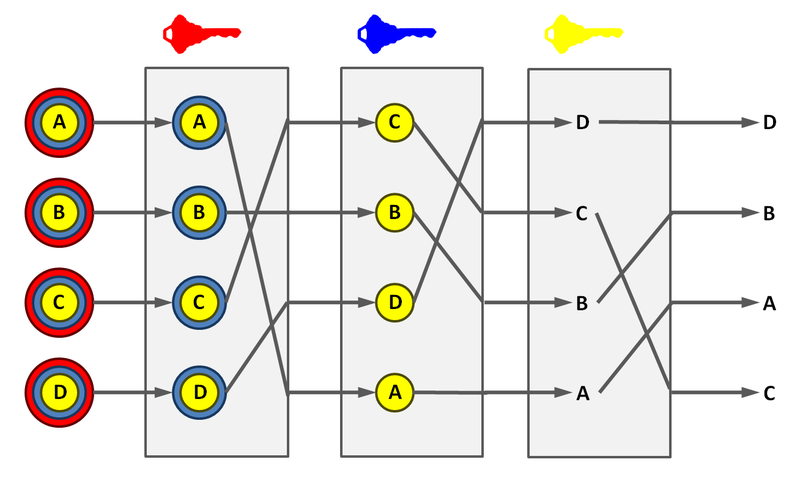
\includegraphics[width=8cm]{cascading}
  \end{center}}
\end{frame}


\begin{frame}
  \frametitle{Mix Network Designs: Mix Networks}

  The second way is to allow users to arbitrarily select which mixes their
  message will pass through, and is what is now generally referred to as a
  \emph{mix network}.

  \uncover<2->{
  \begin{block}{This design has some problems:}
    \begin{itemize}
    \item Berthold, Pfitzmann, and Standtke (2000) argue that mix networks do
      not offer some properties that cascades offer.
    \item<3-> They illustrate a number of attacks to show that, if \emph{only one}
      mix is honest in the network, the anonymity of the messages going
      through it can be compromised.
    \item<4-> These attacks rely on compromised mixes which exploit some
      knowledge of their position in the chain $\dots$
    \item<5-> $\dots$ or multiple messages using the same sequence of mixes
      through the network.
    \end{itemize}
  \end{block}}
\end{frame}


%% XXX fix hanging indentation
\begin{frame}{Background: Mix Networks vs. Anonymous Proxies}
  \begin{columns}[t]
    \column{.5\textwidth}
    \begin{block}{Mix Networks}
      \uncover<2->{
      \small{$\mathbf{+}$} No single point-of-failure \\
        \hspace{2.5mm} (with cascading) \\
      \small{$\mathbf{+}$} Generally strong anonymity guarantees \\
      \small{$\mathbf{+}$} Inbound/outbound traffic analysis \\
        \hspace{2.5mm} does not deanonymise \\
      }
      \uncover<3->{
      \small{$\mathbf{-}$} High latency \\
      \small{$\mathbf{-}$} Slow public-key cryptography
      }
    \end{block}
    \column{.5\textwidth}
     \begin{block}{Anonymous Proxies}
       \uncover<4->{
       \small{$\mathbf{+}$} Low latency \\
       \small{$\mathbf{+}$} Fast, symmetric cryptography \\
       }
       \uncover<5->{
       \small{$\mathbf{-}$} Single point-of-failure \\
       \small{$\mathbf{-}$} No strong anonymity guarantees \\
       \small{$\mathbf{-}$} Inbound/outbound traffic analysis \\
         \hspace{2.5mm} may deanonymise \\
       }
    \end{block}
  \end{columns}
  \vspace*{4mm}
  \uncover<6->{
    \noindent \textbf{Onion Routing: Combine the advantages of each system}
    \begin{itemize}
    \item Use (non-cascading) mix (called a Tor \emph{circuit}) of
      proxies, which are called Tor \emph{relays} or Tor \emph{nodes}
    \item Use asymmetric cryptography for establishing an (one-way) authenticated, encrypted
      channel, then use fast symmetric cryptography.
    \end{itemize}
  }
\end{frame}


\begin{frame}{What is Tor?}
  Tor is an anonymity network, which uses onion routing to encapsulate client traffic in a manner
  such that each node in the client's chosen path only knows the destinations before and after it.
% XXX
\end{frame}


\begin{frame}{How Tor Works: Directory Authorities and Consensus Protocol}
  Tor uses a semi-centralised design, in which certain specific nodes, called
  \emph{Directory Authorities} are trusted ultimately.

  \begin{itemize}
    \item<2-> The Directory Authorities participate in a
      voting protocol to decide upon a canonical decision regarding the nodes within the network.
    \item<3-> They vote upon their views of the network, and eventually derive a \emph{consensus}
      document which is distributed to clients.
    \item<4-> Despite the misleading name, ``consensus'' documents are created by majority vote.
  \end{itemize}
\end{frame}


\begin{frame}{How Tor Works: Consensus Retrieval}
  \begin{block}{Initial Setup}
    \begin{itemize}
      \item<1-> Directory Authority public keys are compiled into the client software.
      \item<2-> Client uses one of these keys to establish an encrypted connection to a
        Directory Authority.
      \item<3-> Client downloads the consensus from the Directory Authority and checks the Directory
        Authorities signatures on the document.
      \item<4-> Client creates a list of all relays within the consensus, weighted by the relays' bandwidths.
      \item<5-> Client chooses a relay from the weighted list to act as its
        \emph{Guard} relay. This Guard will be the client's entry into the network for some set amount
        of time (currently approximately 2 months).
  \end{itemize}
  \end{block}

  \only<6->{
    We currently require that all clients know about all valid nodes in the Tor network, in
    order to safeguard against \emph{partitioning attacks} where an adversary uses a client's
    partial knowledge of the network topology in some manner to gain some advantage (usually to
    increase feasibility of further attacks, e.g. a correlation attack).
  }
\end{frame}


\begin{frame}{How Tor Works: Path Selection}
  % XXX insert description of Tor's current path selection algorithm
  When a new \emph{stream} is created (e.g. some data to be transmitted over Tor has arrived), a
  circuit is either chosen from a list of pre-constructed circuits, or a new circuit is created as
  needed. Using the same bandwidth-weighted list (as before), the Client selects a \emph{Middle}
  relay and an \emph{Exit} relay for the new circuit.
\end{frame}


\begin{frame}
  \frametitle{Establishing a Circuit}
  \only<1-2>{
    \begin{center}
      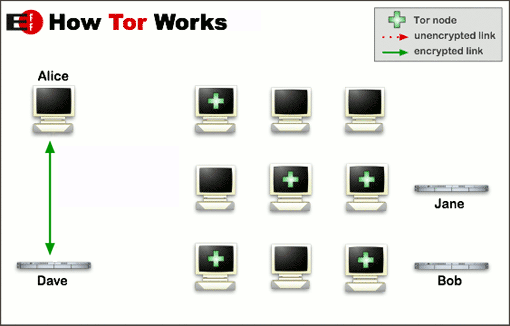
\includegraphics[width=9cm]{tor1}
    \end{center}
    \only<1>{
      Request consensus from Directory Authorities (DirAuths)
    }
    \only<2>{
    Pick entry, middle, and exit node; obtain their public keys from directory
    mirror (DirServ)
    }
  }
  \only<3>{
    \begin{center}
      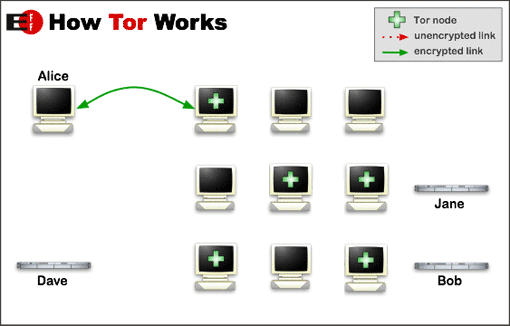
\includegraphics[width=9cm]{tor2}
    \end{center}
    Exchange symmetric key with entry node (Diffie-Hellman)
  }
  \only<4>{
    \begin{center}
      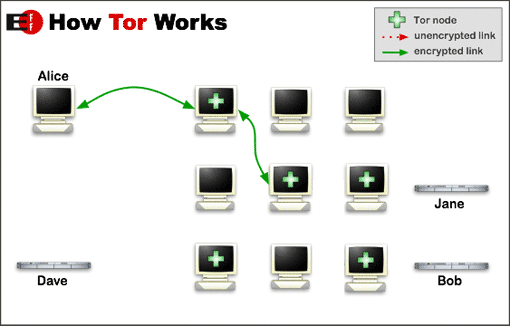
\includegraphics[width=9cm]{tor3}
    \end{center}
    Exchange key with middle node (tunnelled through entry node)
  }
  \only<5>{
    \begin{center}
      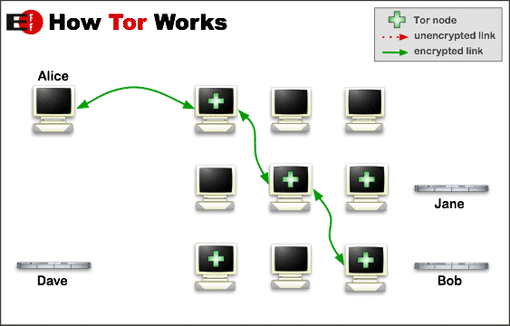
\includegraphics[width=9cm]{tor4}
    \end{center}
    Exchange key with exit node (tunnelled through middle node, tunnelled
    through entry node)
  }
  \only<6>{
    \begin{center}
      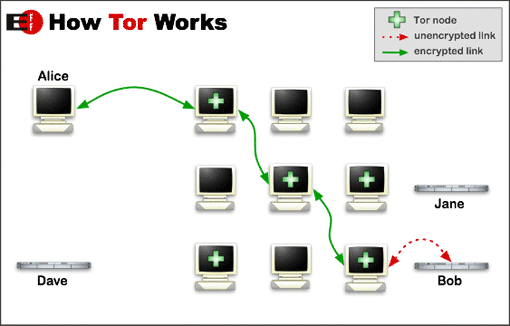
\includegraphics[width=9cm]{tor5}
    \end{center}
    Communicate with Bob
  }
\end{frame}


\begin{frame}{How Tor Works: Circuit construction}
  \begin{block}{Circuit Extension to the Middle Relay}
    \begin{itemize}
      \item<1-> A TLS connection to the Guard $\mathbf{R_1}$ is established, $\mathbf{TLS_{R_1}}$.
      \item<2-> Through $\mathbf{TLS_{R_1}}$, the Client does a circuit-level handshake to setup
        shared keys with the Guard ($\mathbf{R_1}$) for the forward and backward paths,
        $\mathbf{KF_{R_1}}$ and $\mathbf{KB_{R_1}}$ respectively.
      \item<3-> The Client next creates a $\mathbf{RELAY\:EXTEND}$ cell to extend the circuit to the
        Middle relay ($\mathbf{R_2}$) which contains the first stage of the circuit-level handshake
        with $\mathbf{R_2}$. It encrypts this relay cell with $\mathbf{KF_{R_1}}$ and sends it
        forward to $\mathbf{R_1}$, who decrypts with $\mathbf{KF_{R_1}}$ and packages the content
        into a ${\mathbf{RELAY\:CREATE}}$ cell, which is sent over a newly established TLS
        connection between ${R_1}$ and ${R_2}$, $TLS_{R_2}$ who sends its half of the circuit
        handshake in response, packaged in a ${\mathbf{RELAY\:CREATE}}$ cell and reverse encrypted
        (with the corresponding $\mathbf{KB_i}$ keys) down the reverse path.
  \end{itemize}
  \end{block}
\end{frame}


\begin{frame}{How Tor Works: Circuit construction}
  \begin{block}{Circuit Extension to the Exit Relay}
    \begin{itemize}
      \item<1-> After the Client's handshake with the Middle relay ($R_2$) completes, the Client
        creates another $\mathbf{RELAY\:EXTEND}$ cell to extend the circuit to the Exit relay,
        $R_3$.  This is then tunneled over $\mathbf{TLS_{R_2}}$ (which is tunneled through
        $\mathbf{TLS_{R_1}}$). The cell itself is super-encrypted with \\
        $Enc\left(\mathbf{KF_{R_2}}, Enc\left(\mathbf{KF_{R_1}}, \mathbf{CELL}\right)\right)$.
      \item<2-> This cell is sent to $R_1$, who decrypts with $\mathbf{KF_{R_1}}$ and sends it along
        to $R_2$.  $R_2$ decrypts with $\mathbf{KF_{R_2}}$, sees that it's a
        $\mathbf{RELAY\:EXTEND}$ cell to $R_3$, packages the content into a
        ${\mathbf{RELAY\:CREATE}}$ cell (as $R_1$ did before), and sends it to $R_3$.
      \item<3-> The Exit relay $R_3$ receives this ${\mathbf{RELAY\:CREATE}}$ cell, does
        $Dec\left(\mathbf{KF_{R_3}, CELL}\right)$ and receives the traffic the client had intended
        to proxy (which is hopefully further encrypted with some application-layer encryption,
        e.g. TLS, SSH, etc).  
    \end{itemize}
  \end{block}
\end{frame}


\begin{frame}{How Tor Works: Relay Cells on the Forward Path}
  \pgfdeclarelayer{l0}
  \pgfdeclarelayer{l1}
  \pgfdeclarelayer{l2}
  \pgfsetlayers{l0,l1,l2,main}

  \begin{columns}

    \column{.35\textwidth}
    %% XXX how to align right?
    \begin{tikzpicture}
      \path[use as bounding box]
      %  \path[draw] 
      (-6.6,-3.2) rectangle (14.1, 2.2);

      \tikzstyle{box}=[align=center, 
        anchor=north east, minimum height=1cm,
        text height=1.5ex, text depth=.25ex,
      postaction={draw,thin},line width=0cm];

      \only<3->{
        \node[box, minimum width = 3.0cm, minimum height = 2.0cm, fill=gray!40]
        (dest) at (-2,-2)  {Request};
      }
      \only<4->{
        \begin{pgfonlayer}{l2}
          \node[box, minimum height=3.5cm, minimum width=3.5cm, anchor=center, fill=yellow!50] (exit)
          at ([xshift=10mm]$ (dest.north west) !.2! (dest.south east) $) {};
          \node[anchor=north] at (exit.north) {Encrypted with $KF_{R_3}$};
          \node[anchor=north] at ([yshift=-8mm] exit.north) {to \texttt{theintercept.com}};
        \end{pgfonlayer}
      }
      \only<5->{
        \begin{pgfonlayer}{l1}
          \node[box, minimum height=5cm, minimum width=4.0cm, anchor=center, fill=mLightGreen!40] (guard)
          at ([xshift=7mm]$ (exit.north west) !.3! (exit.south east) $) {};
          \node[anchor=north] at (guard.north) {Encrypted with $KF_{R_2}$};
          \node[anchor=north] at ([yshift=-8mm] guard.north) {Sent to $R_3$};
        \end{pgfonlayer}
      }
      \only<6->{
        \begin{pgfonlayer}{l0}
          \node[box, minimum height=6.5cm, minimum width=4.5cm, anchor=center, fill=mLightBrown!40] (entry)
          at ([xshift=4mm]$ (guard.north west) !.4! (guard.south east) $) {};
          \node[anchor=north] at (entry.north) {Encrypted with $KF_{R_1}$};
          \node[anchor=north] at ([yshift=-8mm] entry.north) {Sent to $R_2$};
        \end{pgfonlayer}
      }
    \end{tikzpicture}

    \column{.5\textwidth}
    \begin{itemize}
      \small
      \item Assumption: all relays in the network have well-known public keys
      \item<2-> Use relay public keys to setup an authenticated and encrypted
        channel, which is used to establish symmetric keypairs for the
        \emph{forward} and \emph{reverse paths}:
        \begin{itemize}
          \item Entry relay $R_1$ (keys $KB_{R_1}$, $KF_{R_1}$)
          \item Middle relay $R_2$ (keys $KB_{R_2}$, $KF_{R_2}$)
          \item Exit relay $R_3$ (keys $KB_{R_3}$, $KF_{R_3}$)
        \end{itemize}
      \item<3-> Wants to anonymously send request to \texttt{theintercept.com}
      \item<4-> Prepares Tor \emph{relay cell} as follows:
        \begin{itemize}
          \item<4-> Create request for \texttt{theintercept.com} and encrypt with $KF_{R_3}$
          \item<5-> Set destination as $R_3$ and encrypt with $KF_{R_2}$
          \item<6-> Set destination $R_2$ and encrypt with $KF_{R_1}$
        \end{itemize}
      \item<7-> Send this cell to $R_1$
    \end{itemize}
  \end{columns}
\end{frame}

\addtocounter{framenumber}{-1}
\begin{frame}{How Tor Works: Relay Cells on the Forward Path}
  \pgfdeclarelayer{l0}
  \pgfdeclarelayer{l1}
  \pgfdeclarelayer{l2}
  \pgfsetlayers{l0,l1,l2,main}

  \begin{columns}

    \column{.35\textwidth}
    \begin{tikzpicture}
      \path[use as bounding box]
      %  \path[draw] 
      (-6.6,-3.2) rectangle (14.1, 2.2);

      \tikzstyle{box}=[align=center, 
        anchor=north east, minimum height=1cm,
        text height=1.5ex, text depth=.25ex,
      postaction={draw,thin},line width=0cm];

      \node[box, minimum width = 3.0cm, minimum height = 2.0cm, fill=gray!40]
      (dest) at (-2,-2)  {Request};

      \only<1-5>{
        \begin{pgfonlayer}{l2}
          \node[box, minimum height=3.5cm, minimum width=3.5cm, anchor=center, fill=yellow!50] (exit)
          at ([xshift=10mm]$ (dest.north west) !.2! (dest.south east) $) {};
          \node[anchor=north] at (exit.north) {Encrypted with $KF_{R_3}$};
        \end{pgfonlayer}
      }
      \only<1-6>{
        \node[anchor=north] at ([yshift=-8mm] exit.north) {to \texttt{theintercept.com}};
      }
      \only<1-3>{
        \begin{pgfonlayer}{l1}
          \node[box, minimum height=5cm, minimum width=4.0cm, anchor=center, fill=mLightGreen!40] (guard)
          at ([xshift=7mm]$ (exit.north west) !.3! (exit.south east) $) {};
          \node[anchor=north] at (guard.north) {Encrypted with $KF_{R_2}$};
        \end{pgfonlayer}
      }
      \only<1-4>{
        \node[anchor=north] at ([yshift=-8mm] guard.north) {to $R_3$};
      }
      \only<1>{
        \begin{pgfonlayer}{l0}
          \node[box, minimum height=6.5cm, minimum width=4.5cm, anchor=center, fill=mLightBrown!40] (entry)
          at ([xshift=4mm]$ (guard.north west) !.4! (guard.south east) $) {};
          \node[anchor=north] at (entry.north) {Encrypted with $KF_{R_1}$};
        \end{pgfonlayer}
      }
      \only<1-2>{
        \node[anchor=north] at ([yshift=-8mm] entry.north) {to $R_2$};
      }
    \end{tikzpicture}%

    \column{.5\textwidth}
    \begin{itemize}
      \item $R_1$ receives packet, removes encryption with $KF_{R_1}$
      \item<2-> Sees next destination: $R_2$, forwards
      \item<3-> $R_2$ receives packet, removes encryption with $KF_{R_2}$
      \item<4-> Sees next destination: $R_3$, forwards
      \item<5-> $R_3$ receives packet, removes encryption with $KF_{R_3}$
      \item<6-> Sees next destination: \texttt{theintercept.com}, sends request
    \end{itemize}
  \end{columns}
\end{frame}


\begin{frame}{How Tor Works: Relay Cell on the Reverse Path}
  \pgfdeclarelayer{l0}
  \pgfdeclarelayer{l1}
  \pgfdeclarelayer{l2}
  \pgfsetlayers{l0,l1,l2,main}

  \begin{columns}
    \column{.35\textwidth}
    \begin{tikzpicture}
      \path[use as bounding box]
      %  \path[draw] 
      (-6.6,-3.2) rectangle (14.1, 2.2);

      \tikzstyle{box}=[align=center, 
        anchor=north east, minimum height=1cm,
        %text height=1.5ex, text depth=.25ex,
      postaction={draw,thin},line width=0cm];

      \node[box, minimum width = 3.0cm, minimum height = 2.0cm, fill=gray!40]
      (dest) at (-2,-2)  {Response};

      \only<2-4>{
        \begin{pgfonlayer}{l2}
          \node[box, minimum height=3.5cm, minimum width=3.5cm, anchor=center, fill=yellow!50] (exit)
          at ([xshift=10mm]$ (dest.north west) !.2! (dest.south east) $) {};
          \node[anchor=north] at (exit.north) {Encrypted with $KB_{R_1}$};
        \end{pgfonlayer}
      }
      \only<3-5>{
        \begin{pgfonlayer}{l1}
          \node[box, minimum height=5cm, minimum width=4.0cm, anchor=center, fill=mLightGreen!40] (guard)
          at ([xshift=7mm]$ (exit.north west) !.3! (exit.south east) $) {};
          \node[anchor=north] at (guard.north) {Encrypted with $KB_{R_2}$};
        \end{pgfonlayer}
      }
      \only<4-6>{
        \begin{pgfonlayer}{l0}
          \node[box, minimum height=6.5cm, minimum width=4.5cm, anchor=center, fill=mLightBrown!40] (entry)
          at ([xshift=4mm]$ (guard.north west) !.4! (guard.south east) $) {};
          \node[anchor=north] at (entry.north) {Encrypted with $KB_{R_3}$};
        \end{pgfonlayer}
      }
    \end{tikzpicture}%

    \column{.5\textwidth}
    \begin{itemize}
      \item $R_3$ receives response from \texttt{theintercept.com}.
      \item<2-> $R_3$ encrypts with \\
        $Enc(\mathbf{KB_{R_3}}, Enc(\mathbf{KB_{R_2}}, Enc(\mathbf{KB_{R_1}}, CELL)))$, \\
        and sends to $R_2$.
      \item<5-> $R_2$ decrypts with $\mathbf{KB_{R_3}}$, giving \\
        $Enc(\mathbf{KB_{R_2}}, Enc(\mathbf{KB_{R_1}}, CELL))$, \\
        and sends to $R_1$.
      \item<6-> $R_1$ decrypts with $\mathbf{KB_{R_2}}$, giving \\
        $Enc(\mathbf{KB_{R_1}}, CELL)$, \\
        and sends to the Tor Client.
      \item<7-> The Tor Client decrypts with $\mathbf{KB_{R_1}}$ and thus receives the response.
    \end{itemize}
  \end{columns}
\end{frame}


\section{Tor as Censorship Circumvention Mechanism}

\begin{frame}{Tor as censorship circumvention}
  \begin{itemize}
    \item Various countries filter Internet traffic by destination address
    \item Most prominent example: Great Firewall of China
    \item<2-> Firewalls and gateways cannot see the true destination of Tor traffic
    \item<2-> Tor is a powerful tool to circumvent online censorship (e.g., in China,
      Iran, Turkey, Kazakhstan, Ethiopia, others)
    \item<3-> Can also use Tor to circumvent country filters:
      \begin{itemize}
      \item Need an IP address that isn't in Germany (e.g. because of GEMA
        restrictions on YouTube): can use Tor access YouTube from a non-German
        IP address.
      \end{itemize}
  \end{itemize}
\end{frame}


\begin{frame}{Censorship of Tor}
  \begin{itemize}
    \item Easy solution for censors: 
      \begin{itemize}
        \item<2-> Obtain list of Tor nodes from the Directory Authorities
        \item<3-> Block access to the Tor network (all public relays)
        \item<4-> Even simpler: block access to the Directory Authorities (Iran, Ethopia, Kazakhstan,
          and others have done this historically).
      \end{itemize}
    \item<5-> Solution: Tor Bridges
  \end{itemize}
\end{frame}


\begin{frame}{Tor Bridges}
  \begin{itemize}
    \item<1-> Tor \emph{Bridges} are unpublished entrances to the Tor network used to circumvent
      online censorship when the public relays in the consensus are blocked.
    \item<2-> Bridge IP address and other connection information must be distributed out-of-band.
    \item<3-> Deep Packet Inspection (DPI) or an active adversary is required to identify Bridges.
    \item<4-> Distributed via a centralised system called BridgeDB. Clients can currently obtain
      bridges by:
      \begin{itemize}
        \item visiting \url{https://bridges.torproject.org/}
        \item writing e-mail to \href{mailto:bridges@torproject.org}{bridges@torproject.org}
      \end{itemize}
  \end{itemize}

  \uncover<5->{
    Since 2010, various nation state adversaries have been conducting active probing and enumeration
    attacks to attempt to collect all of Tor's bridges. Since then, an arms race to distribute the
    bridge addresses to honest clients without these adversaries obtaining them has ensued.
  }
\end{frame}


\begin{frame}{Bridge Enumeration Attacks, Part I}
  The first stage of the arms race was to simply identify the ways in which a Tor Client's traffic
  could be distinguished from normal traffic.  This is obviously also effective against
  Tor Bridges.

  \begin{itemize}
    \item<2-> Tor traffic has trivial distiguishers: it's ``disguised'' as TLS traffic, but:
      \begin{itemize}
        \item<3-> It uses random domain names,
        \item<4-> It has a characteristic packet-size distribution,
        \item<5-> Historically, it presents a unique TLS ciphersuite list
      \end{itemize}
  \end{itemize}

  \uncover<6->{
    In 2012, Ethiopia began blocking all TLS (and hence blocking all Tor) traffic by looking for the
    client HELLO.  Any packet with the string $\mathbf{TLS\_DHE\_RSA\_WITH\_AES\_256\_CBC\_SHA}$ in
    it is dropped. If you pick $\mathbf{TLS\_DHE\_RSA\_WITH\_AES\_128\_CBC\_SHA}$ instead, or
    fragment the ciphersuite list, it works anyway.
  }
\end{frame}


\begin{frame}{Bridge Enumeration Attacks, Part I}
  \begin{block}{Since 2010, China's GFW began active probing Tor Bridges, usually in the following manner:}
    \begin{itemize}
    \item<2-> Observe Tor client's TCP connection to the Bridge
    \item<3-> For Tor<0.2.3.17-beta, identification was based upon Tor's unique ciphersuite list
    \item<4-> A seemingly random machine from somewhere in China (possibly using IP-spoofing) will
      connect to the Bridge's IP:port and attempt to complete the first couple steps of the
      handshake
    \item<5-> The Bridge is blocked by IP:port
    \item<6-> The GFW sometimes spoofs a RST from Bridge to the client
    \end{itemize}
  \end{block}

  \uncover<7->{
    \begin{block}{Solution: Tor's Pluggable Transports}
    \end{block}
  }
\end{frame}


\begin{frame}{Pluggable Transports}
  % XXX credit asn, dcf, yawning and others

  In 2011, fellow Tor developer George Kadianakis came up with an idea for a simple SOCKS-proxy
  based API for ``plugging'' obfuscating proxies together, called \emph{Pluggable Transports} (PTs).

  \uncover<2->{
    PTs are generally not meant to provide security benefits, because Tor traffic is tunneled
    through the obfuscating proxy.  Instead, they often provide countermeasures to distinguishers,
    or packet-distribution or timing analysis.
  }
  \begin{itemize}
    \item<3->
      \href{https://www.torproject.org/docs/pluggable-transports.html.en}{Pluggable
        Transport API} allows communication between an obfuscating SOCKS proxy and
        Tor client
  \end{itemize}

  \uncover<4->{
    Currently, the most widely-used and effective Pluggable Transport is obfs4proxy:

    \begin{itemize}
      \item<5-> Created by Yawning Angel.
      \item<6-> It uses Tor's NTor handshake with public keys obfuscated via the Elligator 2 mapping.
      \item<7-> The link layer uses NaCl secret boxes (Poly1305, Xsalsa20).
    \end{itemize}

    \uncover<8->{
      Yawning has recently created a newer PT, called ``basket2'' which uses a hybrid
      handshake between Ed448 Goldilocks and NewHope.
    }
  }
  % XXX PT images from dcf's wiki thing
\end{frame}


\begin{frame}{Pluggable Transports: Magick Potion Ingredients}

  Pluggable Transports are generally considered a ``finished'' research field.  There's an
  incredibly simple formulae for creating one which works, although the ``hard'' problems
  (i.e. distributing the requisite shared secrets) are shoved under the rug.

  \begin{itemize}
    \item<2-> The handshake should be uniform.

    \item<3-> The PT should use some pre-shared key material for server authentication.
    \item<4-> The PT should encrypt starting with the client's first message (i.e. encrypt the first
      stage of the handshake).
    \item<5-> An anthenticated encryption cipher should be used at the transport layer.
  \end{itemize}

  \uncover<6->{
    While there's probably not any remaining research problems in Pluggable Transports for producing
    academic papers, writing new PTs is an incredibly fun project (suitable for Master's, or
    sufficiently-motivated Bachelor's, students) because you get to be super \#yolo and use
    experimental new crypto.
  }

\end{frame}


\begin{frame}{Bridge Enumeration Attacks, Part II}
  While Pluggable Transports effectively obfuscate the link between a Client and a Bridge—and modern
  Pluggable Transports make the traffic data look uniformly indistinguishable from random—this turns
  out to be insufficient to prevent Bridge \emph{enumeration attacks}.

  \only<2->{
    Another possibility is to simply automate obtaining Bridges in the same manner an
    honest client would.
  }
% XXX
\end{frame}


\begin{frame}{A Social Protocol for Bridge Distribution}
  The proposed solution uses attribute-based credentials to record honest users' good behaviour
  (i.e. the bridges not being censored/blocked), which also serves to effectively lock censoring
  adversaries out of the distribution system.

  \uncover<2->{

    %\tiny  % XXX make text size normal?
  Wang, Q., Lin, Z., Borisov, N., \& Hopper, N. (2013, February). \\
  \hspace{2.5mm} rBridge: User Reputation based Tor Bridge Distribution with \\
  \hspace{2.5mm} Privacy Preservation. In NDSS.
  }
\end{frame}
  
\begin{frame}{A Social Protocol for Bridge Distribution}
  \begin{block}{Original rBridge Design}
    \begin{itemize}
      \item<2-> Users are given ``brownie points'' for ``good behaviour''.
      \item<3-> Users with enough brownie points might win the chance to invite their friends.
      \item<4-> Censors lock themselves out of the system via their own bad behaviour.
      \item<5-> Hopefully nobody is friends with the censors enough to give them an invite ticket.
      \item<6-> Some odd crypto choices, minor mistakes, and efficiency sacrifices for very little
        added privacy.
        \begin{itemize}
          \item<7-> K-TAA signature scheme
          \item<8-> Pedersen commitments on vectors
          \item<9-> Oblivious Transfer
          \item<10-> Ad-hoc anonymous credential construction from k-TAA signatures and
            a Camenisch-Stadler NIZK proof-of-discrete-logarithm.
        \end{itemize}
    \end{itemize}
  \end{block}

  \uncover<11->{
    Currently, I'm redesigning the protocol and implementing the scheme using an anonymous
    credential based on algebraic MACs.
  }
\end{frame}


\begin{frame}{A Social Protocol for Bridge Distribution}

  The best game a censor can play against the rBridge scheme is to exhibit good behaviour in order
  to slowly amass brownie points, trading them in for new Bridges and invite tickets. Using an
  \emph{Event-Driven Blocking Strategy}, that is, waiting until some important event, e.g. a
  political protest, and blocking all known Bridges en masse, is the most effective.

  \uncover<2->{
  Some honest users whose Bridges are blocked, and who do not currently posess enough brownie points
  for new, unblocked bridges, will effectively be locked out of the system as collateral damage.
  }

  \uncover<3->{
  \begin{center}
    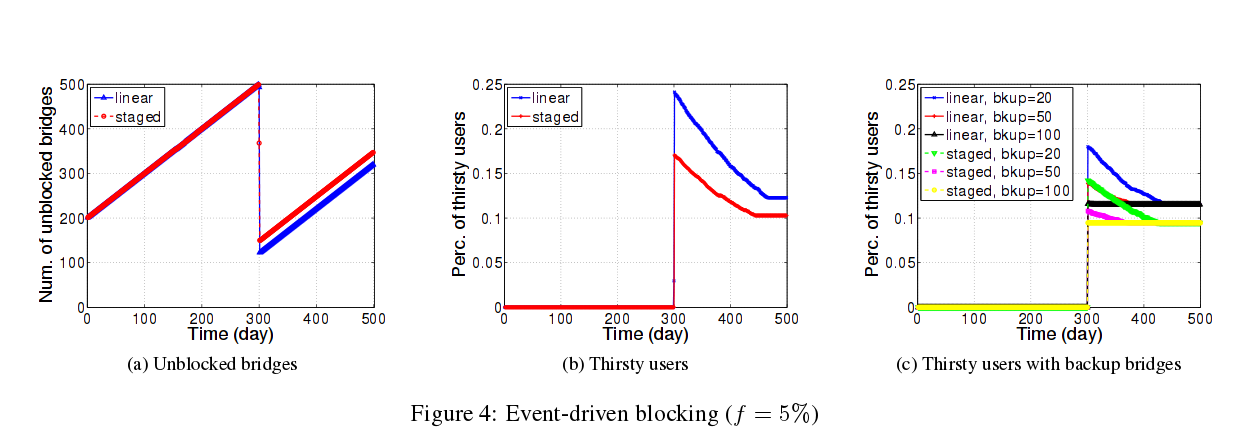
\includegraphics[width=10.5cm]{rbridge}
  \end{center}
  }
\end{frame}


\begin{frame}{Bridge Enumeration Attacks, Part III}
  Even with these measures being implemented, there are other schemes for discovering the locations
  of Tor bridges.

  \uncover<2->{
    Ling, Z., Fu, X., Yu, W., Luo, J., Yang, M. (2011). \\
    \hspace{2.5mm} Extensive Analysis and Large-Scale Empirical Evaluation \\
    \hspace{2.5mm} of Tor Bridge Discovery.
  }

  \uncover<3->{
  \begin{block}{Bridge Enumeration by Running a Middle Relay}
    \begin{itemize}
      \item<4-> Run a Middle relay. Unlike running a Guard or Exit relay, there is no waiting period
        to do this.  Even if you were previously an Exit relay running
      \item<5-> Wait until you see something connecting to you which isn't listed in the consensus.
      \item<6-> Running 20 malicious routers, each with bandwidths of 10MB/s, results in a 90\%
        probability of discovering any one particular Bridge.
      \item<7-> These researchers claim to have run this attack on the live Tor network in 2011,
        enumerating 2369 Bridges in just 14 days.
    \end{itemize}
  \end{block}
  }
\end{frame}


\begin{frame}{Tor proposal \#188: Bridge Guards}

    While we normally tell everyone the a circuit is (normally) three hops, and that a client
    chooses these hops, this is not entirely true.

  \uncover<2->{
  \begin{block}{Tor is loose-source routed}
    \begin{itemize}
      \item<3-> Nothing prevents any relay along the client's chosen path from removing their layer
        of encryption, e.g. $\mathbf{R_1}$ can do
        $Dec(\mathbf{KF_{R_1}}, Enc(\mathbf{KF_{R_2}}, Enc(\mathbf{R_3}, CELL)))$
        to produce
        $Enc(\mathbf{KF_{R_2}}, Enc(\mathbf{R_3}, CELL))$.
      \item<4-> Then re-encrypting $Enc(\mathbf{KF_{R_2}}, Enc(\mathbf{R_3}, CELL))$ to any
        additional relay(s) of its choice.
      \item<5-> Forward this re-encrypted cell to the first additional hop.
      \item<6-> Each additional hop decrypts the cell as usual.
      \item<7-> Eventually, the cell will be fowarded to the client's chosen $\mathbf{R_2}$.
      \item<8-> The client never learns that their traffic traverse additional hops.
    \end{itemize}
  \end{block}
  }

  \uncover<9->{
    We can exploit this unintended feature to give Bridges \emph{their own} Guards, unbeknownst to
    the client, thus protecting Bridges from malicious Middle relays.
  }
\end{frame}


\section{Future Improvements to Tor's Circuit-Level Cryptography}

\begin{frame}{Current Circuit-Level Cryptography}
  Tor currently uses AES256-CTR for the symmetric cryptography at the circuit level.

  \uncover<2->{
  A \emph{Message Authentication Code} (MAC) is recomputed after each cell decryption, that is,
  cells are not end-to-end authenticated from the client.
  }

  \uncover<3->{
  Although we've never witnessed an adversary take advantage of any of these, there are various
  known potentential issues.
  }

  \uncover<4->{
  Due to using CTR mode and re-MACing at each hop, a tagging attacks is possible.
  }
\end{frame}


\begin{frame}{A Known Tagging Attack on Tor's Circuit-Level Cryptography}
  Assumption: the Guard relay is controlled by an adversary, who also controls (some) Exit relay(s).

  \begin{itemize}
    \item<2-> When receiving cells from the target client, the Guard XORs a \emph{tag} (e.g. some
      bits) into the decrypted cell, recalculates the MAC, and forwards to the Middle relay.
    \item<3-> The Middle relay successfully verifies the MAC, decrypts the cell, computes a new
      MAC, and forwards to the Exit relay.
    \item<4-> The Exit relay successfully verifies the MAC, and
    \item<5-> If the chosen Exit happens to be adversary-controlled:
      \begin{itemize}
      \item<6-> The Exit attempts to XOR the same tag back out, effectively removing it, then
        decrypts to produce the original cell.
      \item<7-> The adversary has now confirmed that she is both the Guard and the Exit for the
        client's circuit.
      \end{itemize}
    \item<8-> Otherwise, if the Exit is not colluding with the Guard:
      \begin{itemize}
      \item<9-> The Exit decrypts the cell to produce garbage.
      \item<10-> The Tor Protocol says that the Exit $\mathbf{MUST}$ now send a
        $\mathbf{RELAY\:END}$ cell to tear down the circuit, and hence
      \end{itemize}
      \item<11-> The adversary may repeat this attack until a colluding Exit relay is chosen
        by the client.
    \end{itemize}
\end{frame}

\begin{frame}{(Needed!) Future Improvements to Tor's Circuit-Level Cryptography}

  We would like to switch to using a chained, authenticated encryption, 509-byte wide block cipher.

  \uncover<2->{
    Doing so renders changes to a cell at any hop detectable.
  }

  \uncover<3->{
    There isn't such a cipher yet.
  }
  \uncover<4->{
    \begin{block}{Other potential (non-cryptographic) improvements to Tor's circuit protocol:}

  There's not really any reasons we haven't considered disparate forward and reverse paths.  Nothing
  in the crypto or protocol is technically preventing it.  It would be an interesting area of
  research to see the changes (and, hopefully, improvements to anonymity guarantees) which might be
  derived from disjoint path selection.
    \end{block}
  }
\end{frame}

\section{Tor Relay Handshake}

\begin{frame}{Tor's Relay Handshake Protocol: NTor}
  Tor's current handshake, NTor, is a one-way-authenticated, Diffie-Hellman based handshake which
  uses X25519.

  \uncover<2->{
    In the event of a quantum-capable adversary in the future, who is currently recording Tor
    handshakes now, we need a post-quantum handshake.
  }
\end{frame}


\begin{frame}{Proposed Post-Quantum Hybrid Handshakes for Tor}
  \begin{block}{A Modular Hybrid Handshake}
    Tor proposal \#269: Transitionally secure hybrid handshakes \\
    by John Schanck, William Whyte, Zhenfei Zhang.

    \begin{itemize}
      \item<2-> Created by John Schanck, William Whyte, Zhenfei Zhang.
      \item<3-> Allows for composition of a classical handshake, e.g. Tor's current NTor handshake,
        with a key encapsulation mechanism (KEM) which is believed to be post-quantum secure.
      \item<4-> Currently proposed post-quantum KEMs are:
        \begin{itemize}
          \item<5-> Tor proposal \#263: NTRU
          \item<6-> Tor proposal \#270: NewHope
        \end{itemize}
    \end{itemize}
  \end{block}

  \uncover<7->{
    John Schanck currently has a branch which integrates NTRU, and I'm currently working on an
    expirmental branch which implements the modular hybrid handshake (\#269) and adds a plugin to
    implement the NewHope version (\#270).
  }
\end{frame}

\begin{frame}{Questions \& Contact}
  \begin{center}
  Isis Agora Lovecruft\\
  isis@torproject.org \\
  0A6A 58A1 4B59 46AB DE18  E207 A3AD B67A 2CDB 8B35
  \end{center}
\end{frame}

\end{document}
